%!TeX program = xelatex
%Do not change
\documentclass[12pt, oneside]{article}
\usepackage{amssymb,amsmath}
\usepackage[margin=1in]{geometry}
\usepackage{textpos}
\usepackage{float}
%\usepackage{color}
\usepackage{graphicx}
\usepackage[inter-unit-product =\cdot]{siunitx}
\let\DeclareUSUnit\DeclareSIUnit
\let\US\SI
\DeclareUSUnit\inch{in}
\DeclareUSUnit\foot{ft}
\DeclareUSUnit\mile{mi}
\DeclareUSUnit\foot{ft}
\DeclareUSUnit\slug{slug}
\DeclareUSUnit\pound{lb}
%\usepackage{tikz}
%\usetikzlibrary{positioning}
%\usepackage{tikz-3dplot}
%\usepackage{pgfopts}
%\usepackage{wasysym}
%\usepackage{stanli}

% You may add the packages you need here
\begin{document}

%TODO change numbers in problems
\begin{textblock*}{4cm}(-1.7cm,-2.3cm)
\noindent {\scriptsize AE333 Fall 2021}
\end{textblock*}

%Do not modify other than typing your acknowledgement where stated
\begin{textblock*}{13.5cm}(-1.7cm,-1.8cm)
%\noindent \textit{\footnotesize Acknowledgement: Your acknowledgement for collaboration and other sources goes here. }
\end{textblock*}

\vspace{1cm}

%Do not modify other than typing the homework number after #
\begin{center}
\textbf{\Large Homework 1 Solution}
\end{center}

%Rest should contain your solution for the homework. Feel free to improvise in ways that you believe make grading easier.
\begin{enumerate}
	\item %1-16
		Find the internal load at points D and E.
		\begin{figure}[H]
			\centering
			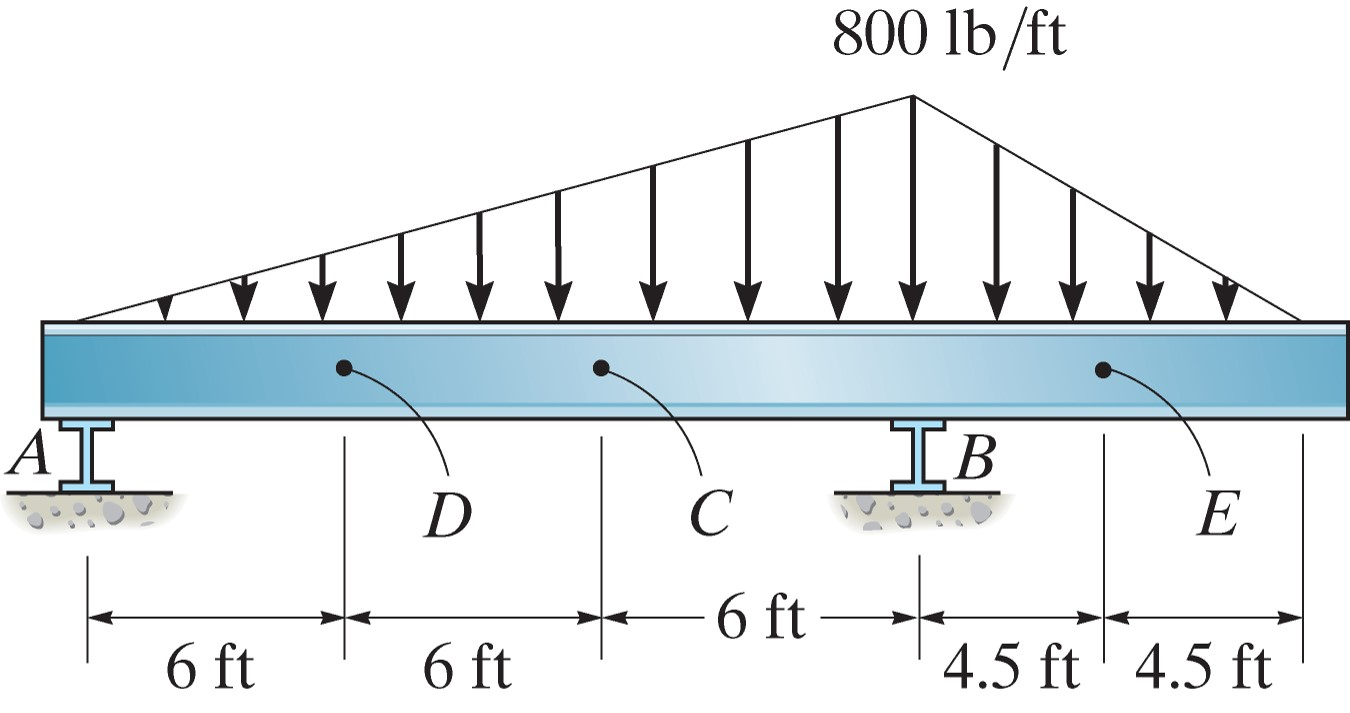
\includegraphics[width=0.6\linewidth]{beam}
			\label{fig:beam}
		\end{figure}
		\begin{itemize}
			\begin{figure}[H]
				\centering
				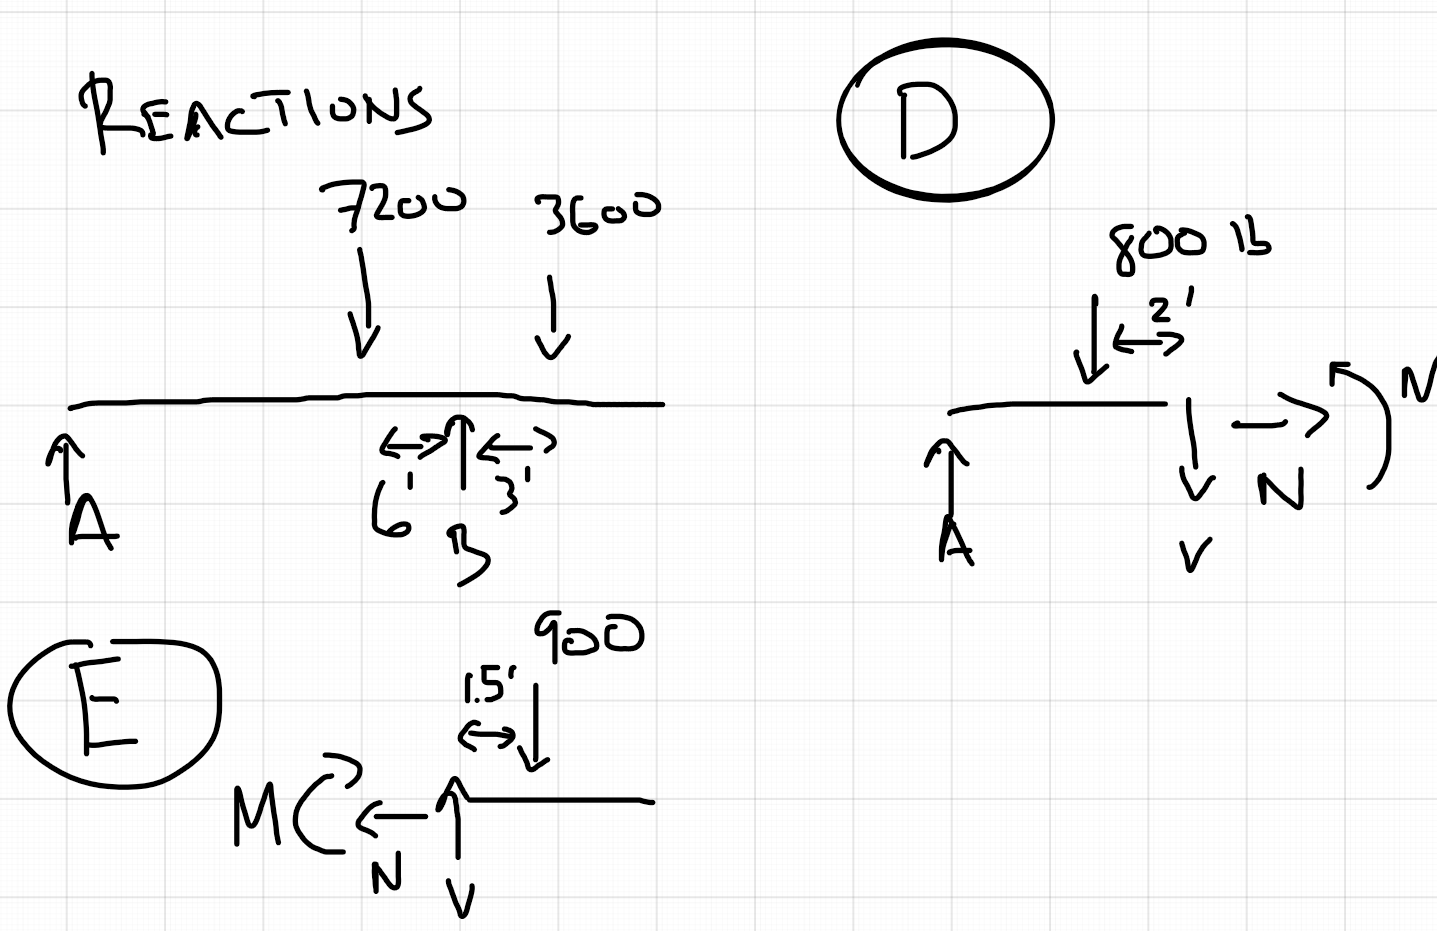
\includegraphics[width=0.7\linewidth]{hw1-1}
			\end{figure}
			\item In this problem we will need to solve for the reaction forces. We could find internal forces at $E$ without any reactions, but since we will need them for internal forces at $D$, we start by finding them.
			\begin{align*}
				\sum F_x &= 0 = A+B - 7200 - 3600\\
				\sum M_B &= 0 = -3(3600) + 6(7200) - 18 A\\
				A &= 1800\text{ lb }\\
				B &= 9000\text{ lb }
			\end{align*}
		\item We start by cutting a section at D, considering the left side since there are fewer terms. NOTE: we must recalculate the force for the distributed load, since $D$ occurs 1/3 of the length of the linearly distributed load, we find the force is $(800/3 \text{ lb/ft})(6 \text{ ft})(1/2)$
			\begin{align*}
				\sum F_x &= 0 = N\\
				\sum F_y &= 0 = 1800 - 800 - V\\
				\sum M_D &= 0 = M + 800(2) - 1800(6)\\
				N &= 0 \text{ lb}\\
				V &= 1000\text{ lb}\\
				M &= 9200\text{ ft lb}
			\end{align*}
		\item Next we cut a section at E, this time considering the right-hand side.
			\begin{align*}
				\sum F_x &= 0 = -N\\
				\sum F_y &= V - 900\\
				\sum M_E &= -M -900(1.5)\\
				N &= 0 \text{ lb }\\
				V &= 900 \text{ lb } \\
				M &= -1350 \text{ ft lb }
			\end{align*}
		\end{itemize}
	
	\item %1-14
		A hacksaw (and many other styles of thin-bladed saws) are held stiff via a pretensioning as shown.
		For a pre-load force of 120 N, find the internal loading acting on section $b-b$ through point $D$.
		\begin{figure}[H]
			\centering
			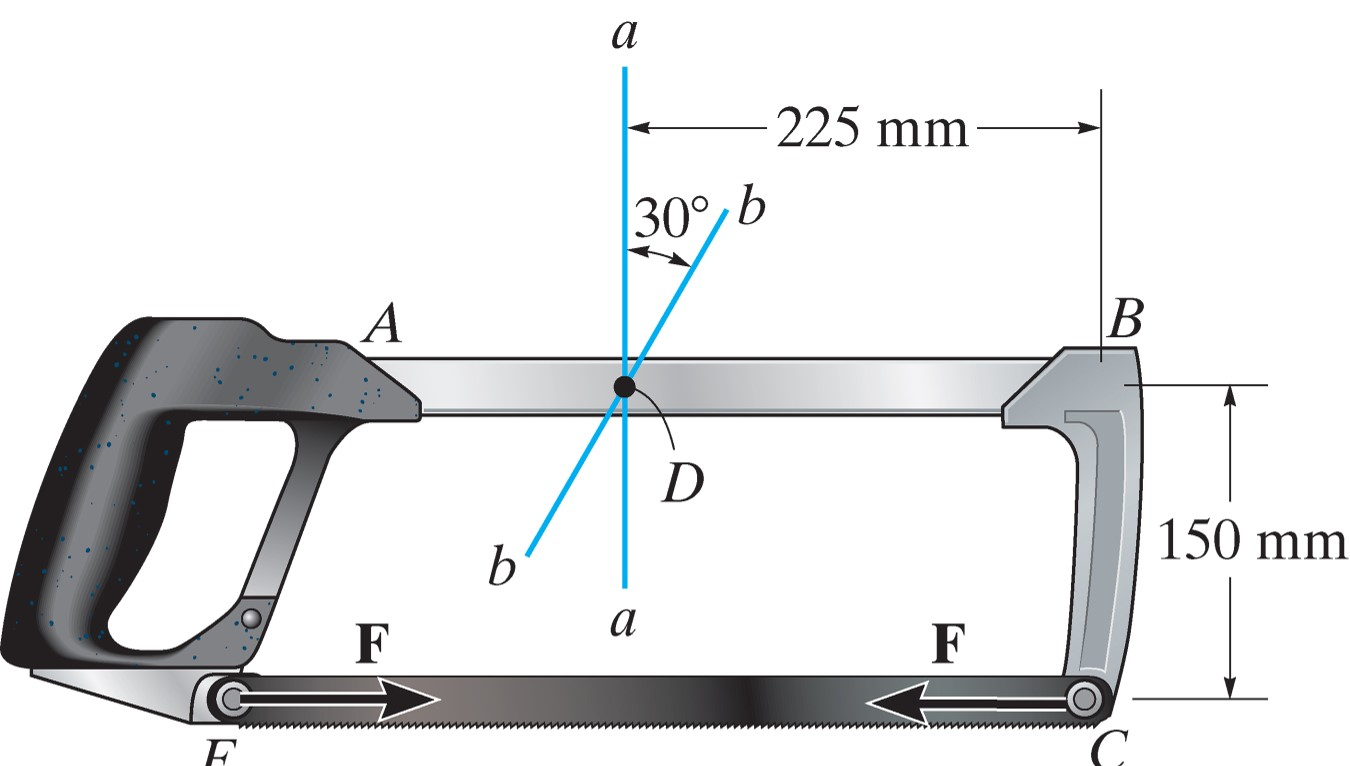
\includegraphics[width=0.6\linewidth]{hacksaw}
			\label{fig:hacksaw}
		\end{figure}
		\begin{itemize}
			\item We start by sectioning the right side of the hacksaw. In order to more conveniently find the internal forces along the angled section we set up a rotated coordinate system.
			\item Separating $F$ into its $x$ and $y$ components we find $F_x = 120 \cos 30$ and $F_y = 120 \sin 30$
			\item Before we solve for internal forces, we notice that the end of the hacksaw aligns with the $x$ axis, so we only need to consider the $y$ component of force in the moment calculations.
			\begin{align*}
				\sum F_x &= 0 = -N - 120 \cos 30 \\
				\sum F_y &= 0 = V - 120 \sin 30 \\
        \sum M_b &= 0 = -120 \sin 30 \sqrt{225^2+150^2}- M\\
				N &= \SI{-104}{N}\\
				V &= \SI{60}{N}\\
        M &= \SI{-16200}{N.mm} = \SI{-16.2}{N.m}
			\end{align*}
			\begin{figure}[H]
				\centering
				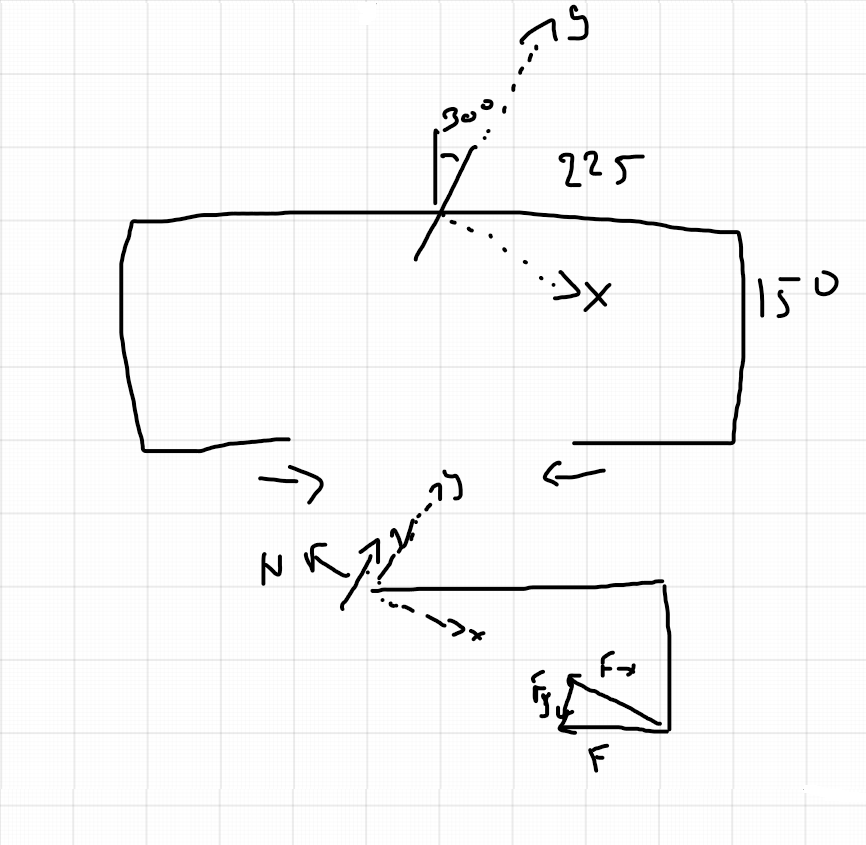
\includegraphics[width=0.7\linewidth]{hw1-2}
			\end{figure}
		\end{itemize}

	\item %1-28
		A bit brace is a type of hand drill.
		If the brace shown jams and is subjected to the force shown, find the resultant internal loading on the shank of the drill bit (point A).
		\begin{figure}[H]
			\centering
			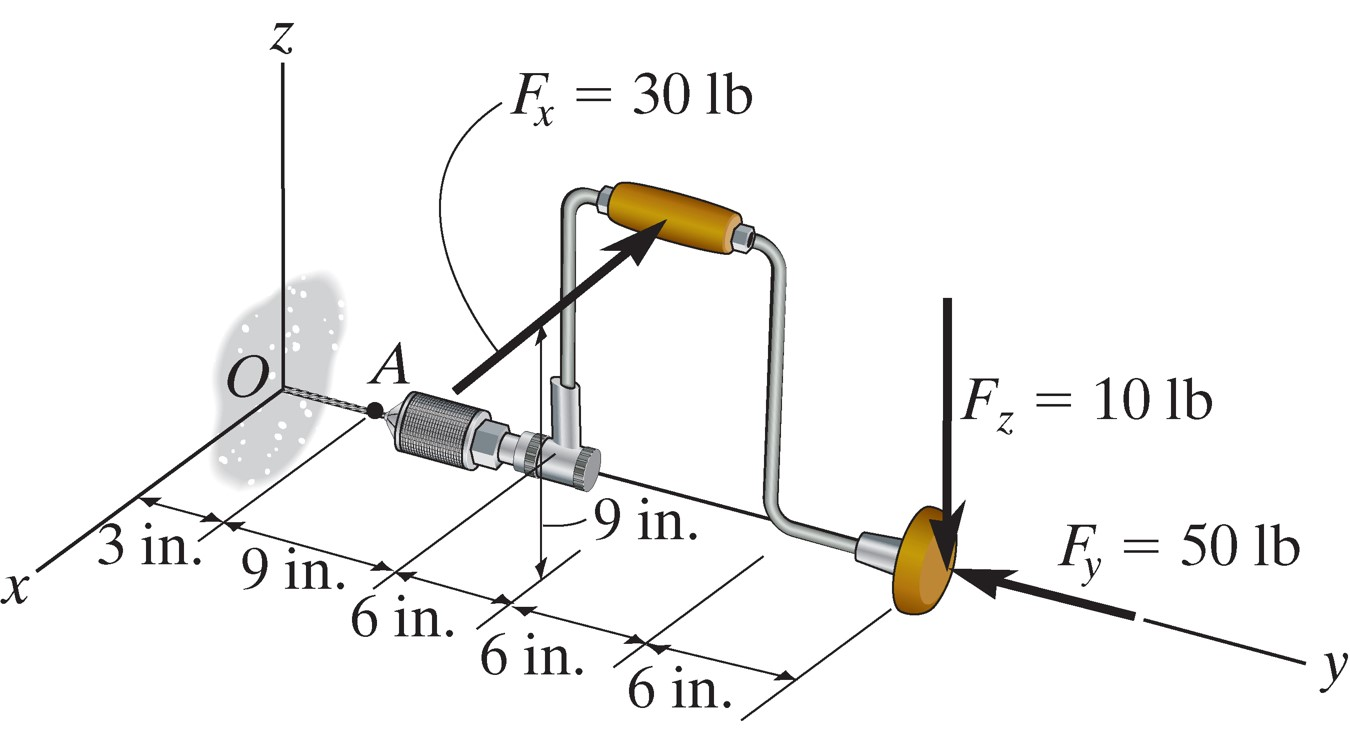
\includegraphics[width=0.6\linewidth]{brace}
			\label{fig:brace}
		\end{figure}
		\begin{itemize}
			\item In this case if we section the drill bit we do not need to find any reaction forces, so we make our section and consider all 6 force and moment equations.
			\begin{figure}[H]
				\centering
				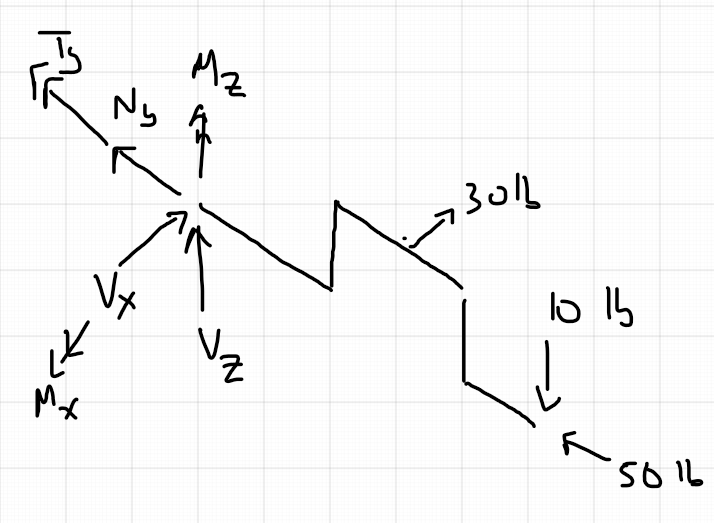
\includegraphics[width=0.7\linewidth]{hw1-3}
			\end{figure}
			\begin{align*}
				\sum F_x &= 0 = -V_x - 30\\
				\sum F_y &= 0 = -N_y - 50\\
				\sum F_z &= 0 = V_z - 10\\
				\sum M_x &= 0 = M_x - 27(10)\\
				\sum M_y &= 0 = -T_y -9(30)\\
				\sum M_z &= 0 = M_z 15(30)\\
				V_x &= \US{-30}{lb}\\
				N_y &= \US{-50}{lb}\\
				V_z &= \US{10}{lb}\\
				M_x &= \US{270}{in.lb}\\
				T_y &= \US{-270}{in.lb}\\
				M_z &= \US{-450}{in.lb}\\
			\end{align*}
		\end{itemize}

	\item %1-32
		Determine the largest uniform load, $w$, that can be applied to the frame shown without exceeding an average tensile stress of $\sigma = \SI{15}{MPa}$ or an average shear stress of $\tau = \SI{16}{MPA}$ along section $b-b$.
		The bars shown are square tubes $\SI{45}{mm}$ on the outside and $\SI{35}{mm}$ on the inside.
		\begin{figure}[H]
			\centering
			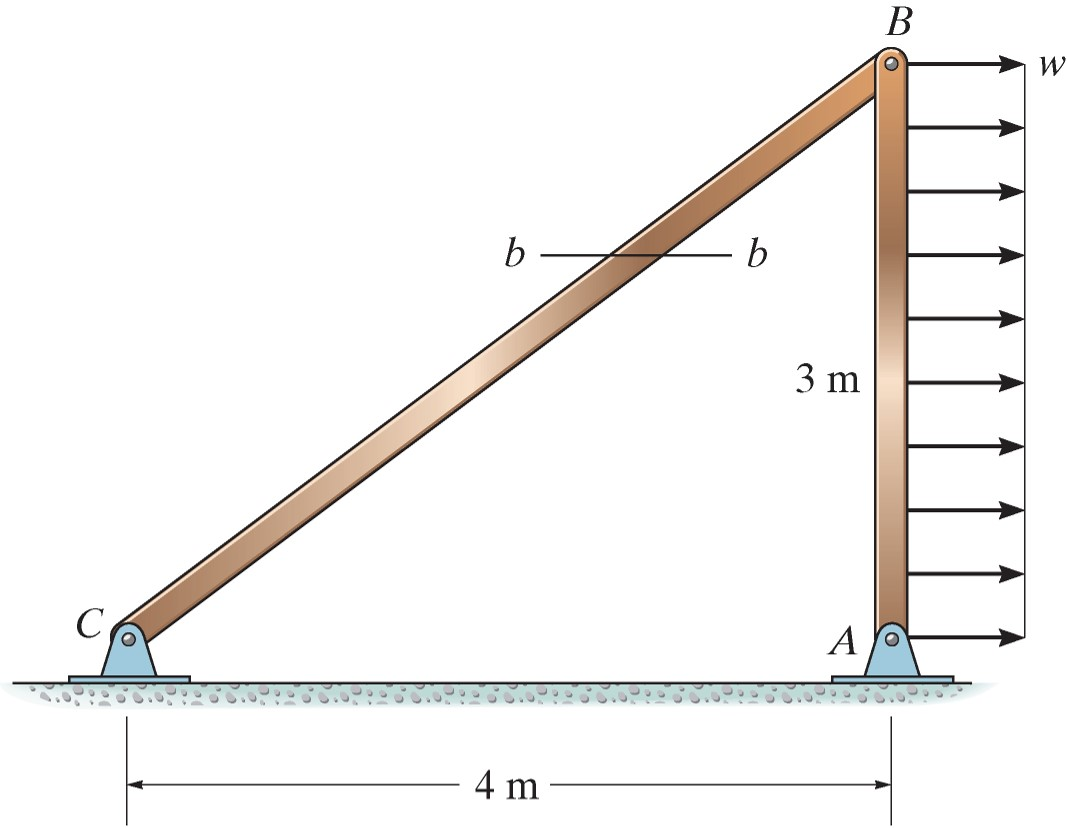
\includegraphics[width=0.6\linewidth]{truss}
			\label{fig:truss}
		\end{figure}
		\begin{itemize}
			\item Since the only forces applied to the member $BC$ occur through pins at the ends, this is a two-force member, which means both forces must act along the member (pure tension/compression) for it to remain in static equilibrium.
				\begin{figure}[H]
					\centering
					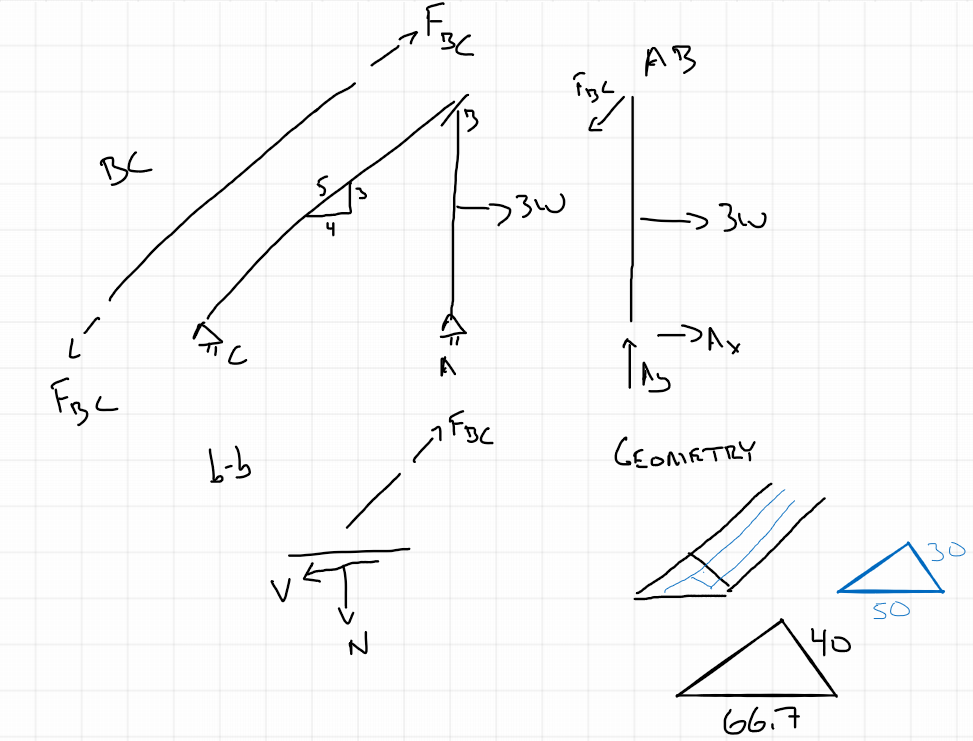
\includegraphics[width=0.7\linewidth]{hw1-4}
				\end{figure}
			\item Knowing the direction of the force allows for us to solve for it directly by considering the moment equilibrium about point $A$ of a section of the member $AB$.
			\begin{align*}
				\sum M_A &= 0 = -3w(1.5) + \frac{4}{5} F_{BC}(3)\\
				F_{BC} &= 1.875w
			\end{align*}
		\item Next we consider the section $b-b$, to find the forces $N$ and $V$ we must separate $F_{BC}$ into normal and shear components and we find
			\begin{align*}
				N &= \frac{3}{5} F_{BC} = 1.125w\\
				V &= \frac{4}{5} F_{BC} = 1.5w
			\end{align*}
		\item We must also adjust the area of our segment as shown since the angled cut will be different than a perpendicular cut. 
      We can use geometry from the sketch, $A = (45)(45)(5/3) - (35)(35)(5/3) = \SI{1333}{mm^2}$, which now allows us to solve for $w$ in both shear and tension.
			\begin{align*}
				\tau &= V/A = \SI{16}{MPa}\\
				\sigma &= N/A = \SI{15}{MPa}\\
				w_\tau &= \SI{14.2}{kN/m}\\
				w_\sigma &= \SI{17.8}{kN/m}
			\end{align*}
		\item We choose the lesser of these (meaning shear failure will occur first) and find $w=\SI{14.2}{kN/m}$.
		\end{itemize}
	
	\item %1-54
		Two members for an airframe are welded together using a $30^\circ$ fish-mouth weld.
		Find the average shear stress on the plane of each weld for the case shown.
		\begin{figure}[H]
			\centering
			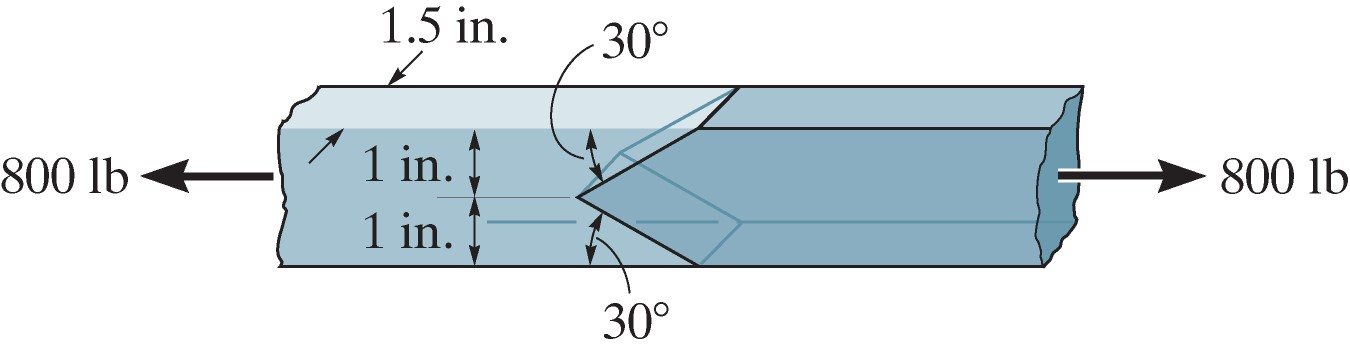
\includegraphics[width=0.6\linewidth]{fish-mouth}
			\label{fig:fish-mouth}
		\end{figure}
		\begin{itemize}
			\begin{figure}[H]
				\centering
				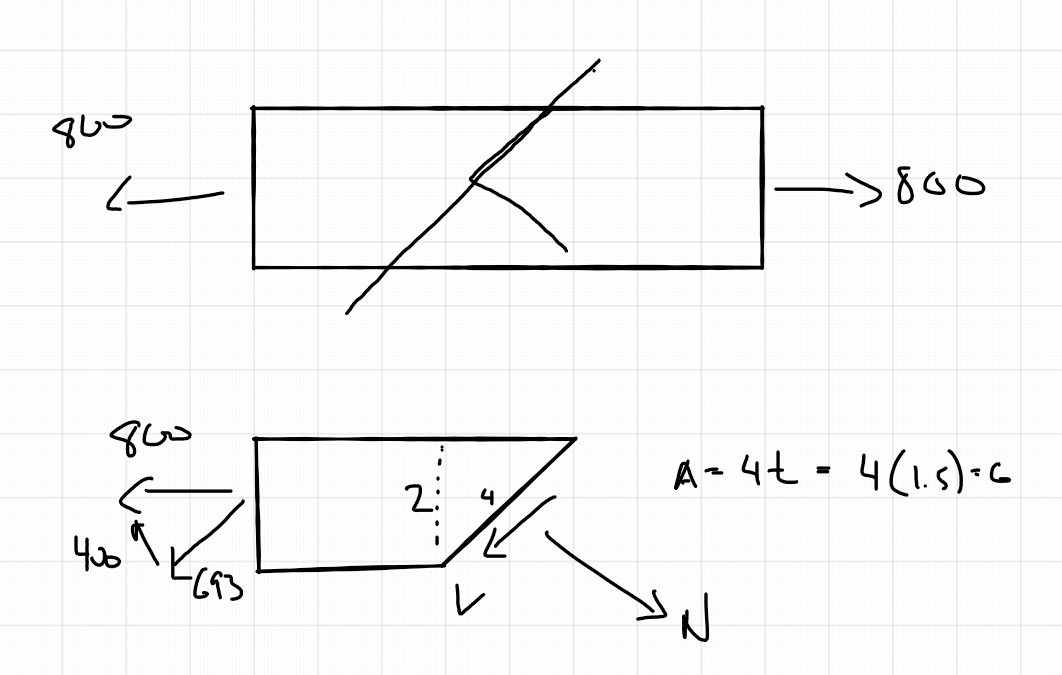
\includegraphics[width=0.7\linewidth]{hw1-5}
			\end{figure}
			\item Since the part is symmetric, we actually don't need to make complicated sections, we can consider one 30 degree section following one half of the weld.
			\item As we have with other problems, we will need to split the 800 lb horizontal force into the coordinate system that aligns with our weld section cut. After that is done we can use equilibrium to solve for the normal and shear force.
			\begin{align*}
				\sum F_x &= 0 = N - 800 \sin 30\\
				\sum F_y &= 0 = -V - 800 \cos 30\\
				N &= \US{400}{lb}\\
				V &= \US{-693}{lb}
			\end{align*}
		\item With the forces found, we can now find the shear stress. We need to use geometry to find the cross sectional area, $A = 4(1.5) = \US{6}{in^2}$ which gives a shear stress of $\tau = \US{115}{ksi}$
		\end{itemize}

	\item %1-86
		Two aluminum rods support a vertical force of $P=\SI{25}{kN}$.
		Find the diameter of the rods (they are solid and have the same diameter) for a failure stress of $\sigma=\SI{120}{MPa}$ and a safety factor of 1.5.
		\begin{figure}[H]
			\centering
			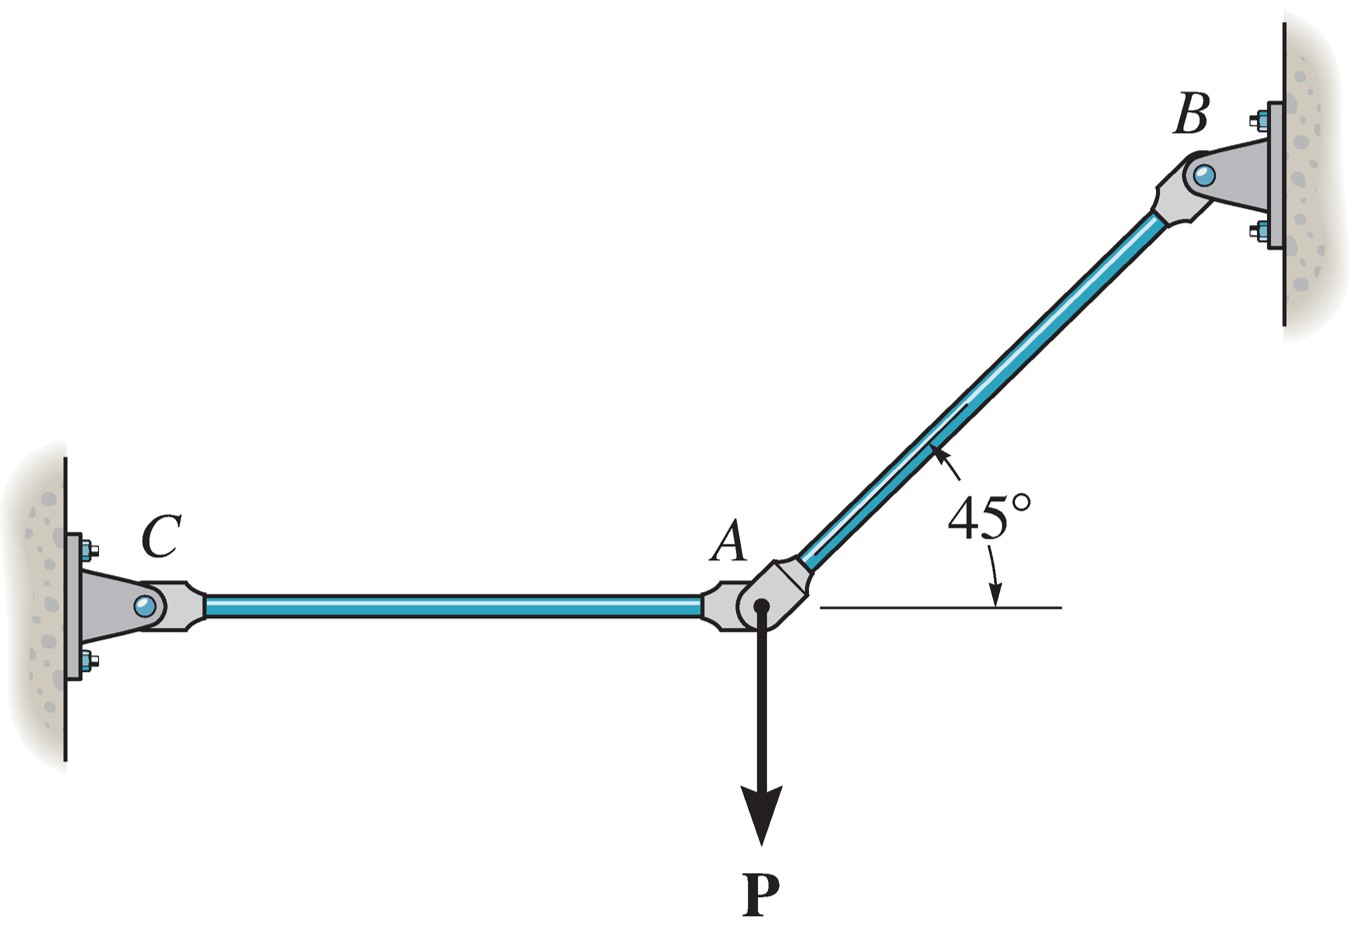
\includegraphics[width=0.6\linewidth]{rods}
			\label{fig:rods}
		\end{figure}
		\begin{itemize}
			\begin{figure}[H]
				\centering
				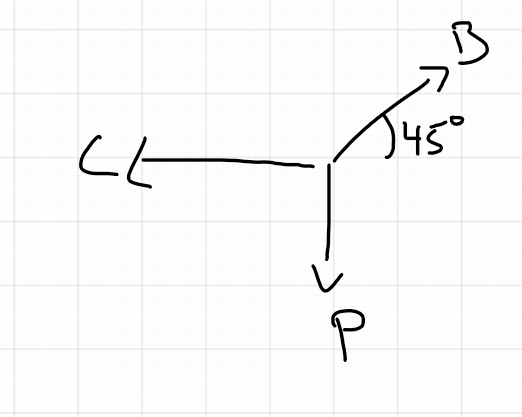
\includegraphics[width=0.7\linewidth]{hw1-6}
			\end{figure}
			\item Since both rods only have pin supports and connections, we can once again use the two-force member shortcut, and we know that all forces in the rods will need to act along the axis of the rods. With this knowledge and a free body diagram we can proceed to the equilibrium equations.
			\begin{align*}
				\sum F_x &= 0 = -C + B \cos 45\\
				\sum F_y &= 0 = -P + B \sin 45\\
				B &= \sqrt{2} P = \SI{35.4}{kN}\\
				C &= P = \SI{25}{kN}
			\end{align*}
		\item We can now use the given material properties and safety factor to find the needed diameters for each rod
			\begin{align*}
				FS &= 1.4 = \frac{\sigma_{fail}}{\sigma_{allow}} = \frac{\SI{130}{MPa}}{F/A}\\
				A &= \pi (d/2)^2 = \frac{\pi}{4}d^2\\
				d_B &= \SI{22.0}{mm}\\
				d_C &= \SI{18.5}{mm}
			\end{align*}
		\item Since the problem stated that the rods have the same diameter, we choose the larger diameter to ensure that both rods meet the required safety factor
		\end{itemize}

	\item %1-93
		The two rods ($AB$ and $CD$) supporting beam $AC$ are made of steel.
		Determine the smallest rod diameter to support the dead loads shown along with an additional live load of $\SI{5}{kN}$.
		The resistance factor for steel in tension is $\phi=0.8$, use a dead load factor of $\gamma_D = 1.3$ and a live load factor of $\gamma_L = 1.8$.
		The failure stress for this steel alloy is $\sigma_{fail} = \SI{340}{MPa}$.
		\begin{figure}[H]
			\centering
			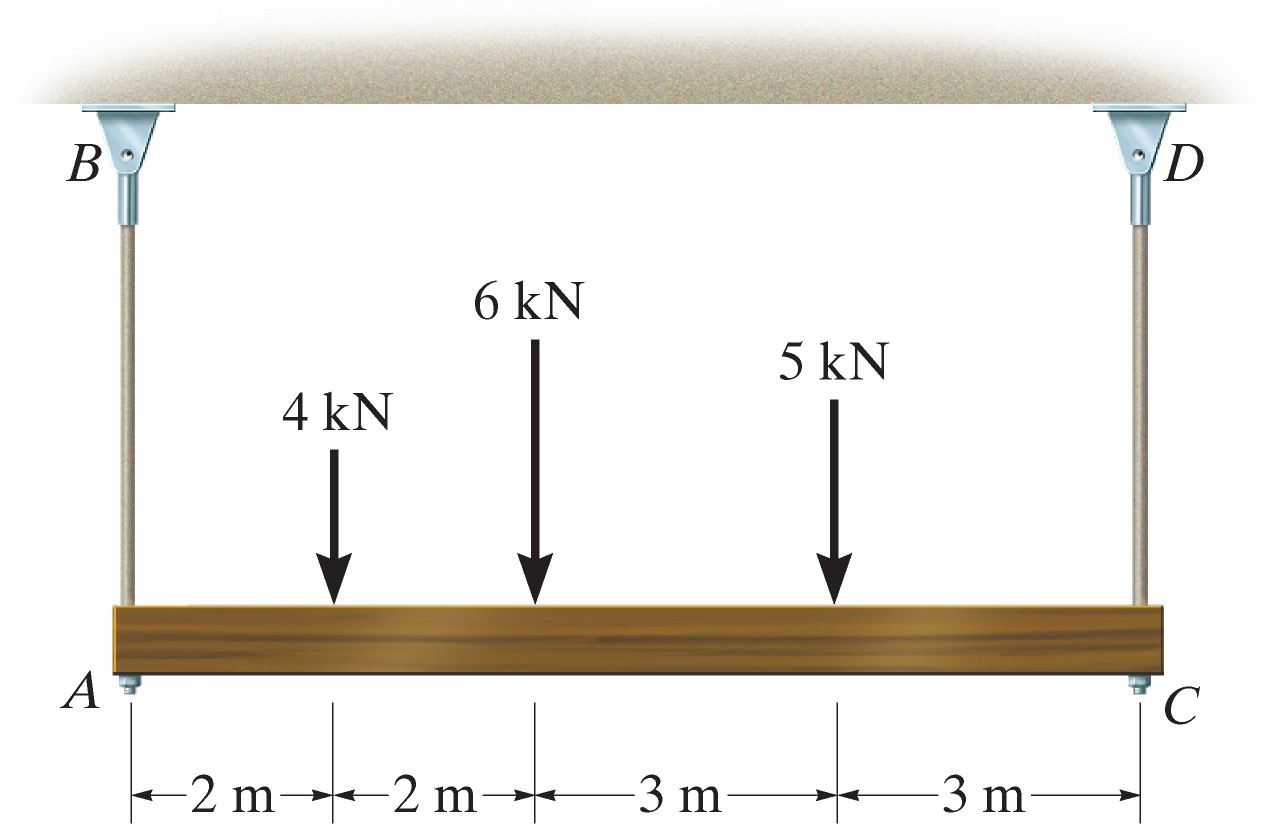
\includegraphics[width=0.6\linewidth]{hangingbeam}
			\label{fig:hangingbeam}
		\end{figure}
		\begin{itemize}
			\item In this problem, it is most convenient to apply the load factors to each load before we proceed with solving the static equilibrium equations.
			\begin{figure}[H]
				\centering
				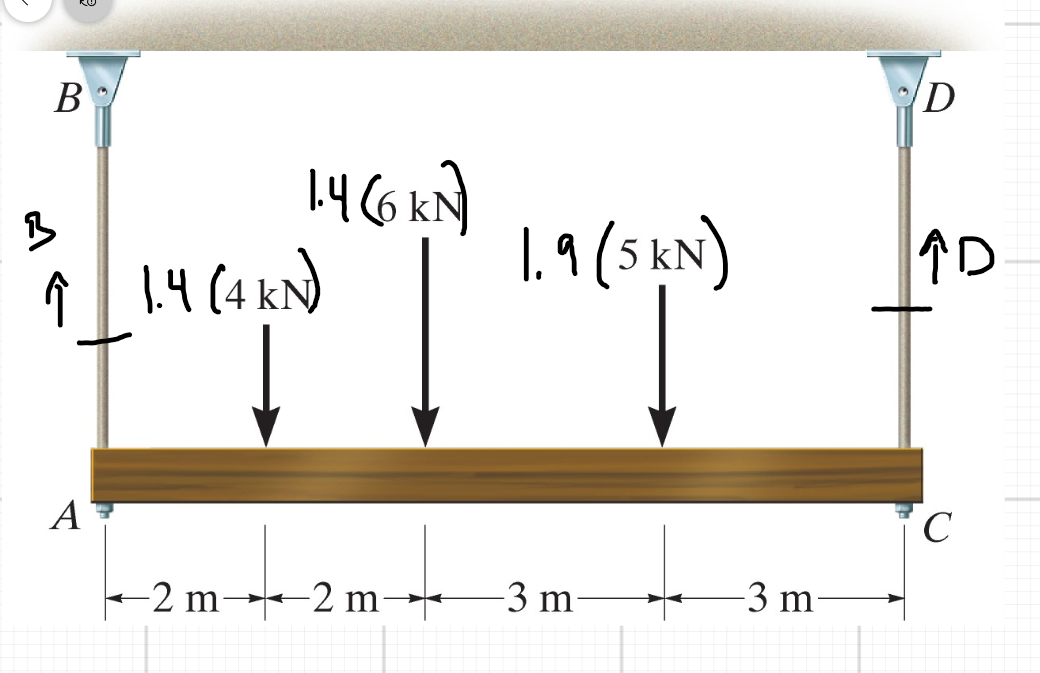
\includegraphics[width=0.7\linewidth]{hw1-7}
			\end{figure}
		\item The static equilibrium equations are then
		\begin{align*}
			\sum F_x &= 0\\
			\sum F_y &= 0 = B - 1.3(4) - 1.3(6) - 1.8(5) + D\\
			\sum M_B &= 0 = -1.3(4)(2) - 1.3(6)(4) - 1.8(5)(7) + D(10)\\
			D &= \SI{10.46}{kN}\\
			B &= \SI{11.54}{kN}
		\end{align*}
	\item We can proceed to find the diameter by setting the stresses from the forces $B$ and $D$ equal to the resistance factor multiplied by the failure stress
		\begin{align*}
			0.9(\SI{340}{MPa}) &= F/A = \frac{F}{\pi/4 d^2}\\
			d &= \sqrt{\frac{4F}{\pi (0.8)(\SI{340}{MPa})}}\\
			d_B &= \SI{7.00}{mm}\\
			d_D &= \SI{7.35}{mm}
		\end{align*}
		\end{itemize}

	\item %C1-1
		Extreme high winds can cause failure of highway signs, as shown here.
		Assuming a uniform wind pressure of $\SI{4}{kPa}$, estimate reasonable sign dimensions and determine the resultant shear where the failure occurred.
		Compare your answer with the material properties listed on the back cover of your textbook (or an online database), does this seem like a reasonable failure or do you suspect some bad assumptions?
		\begin{figure}[H]
			\centering
			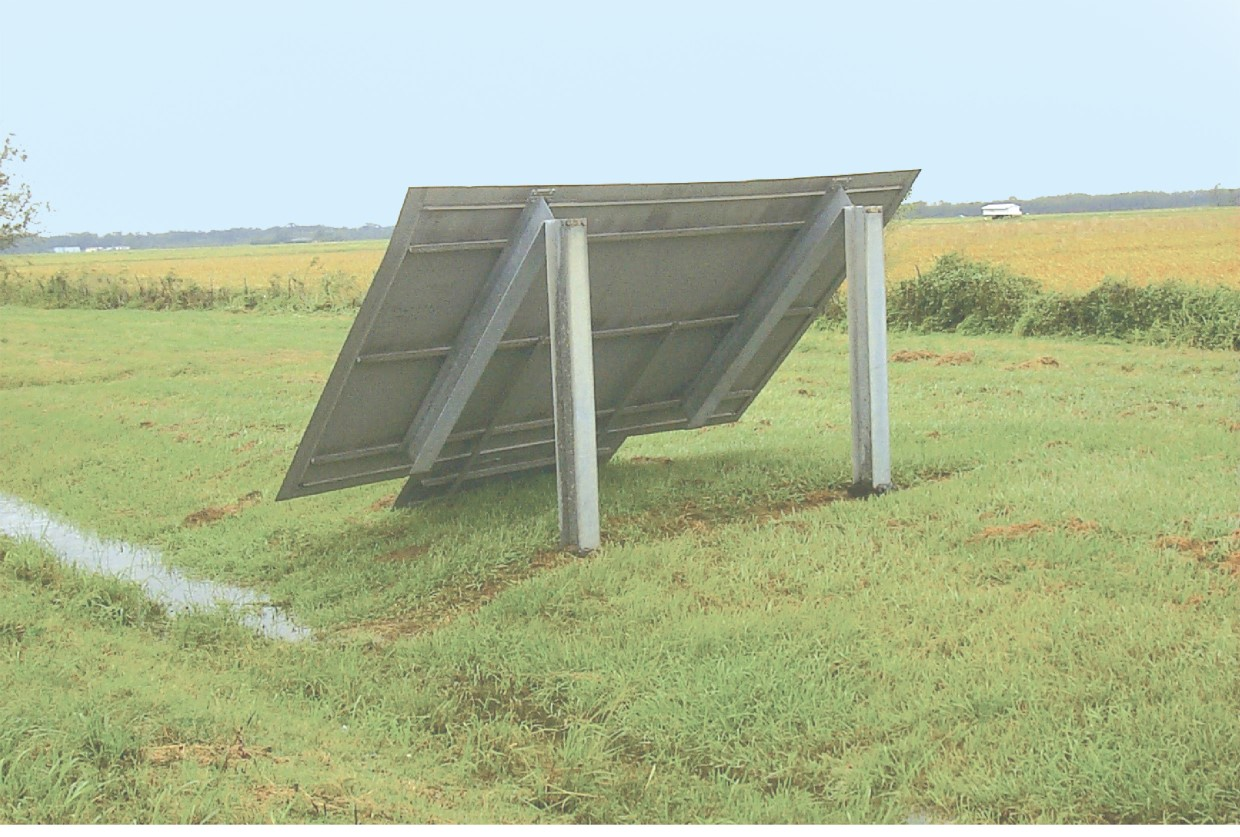
\includegraphics[width=0.6\linewidth]{sign}
			\label{fig:sign}
		\end{figure}
		\begin{itemize}
			\item For this problem I assumed a sign that was $\SI{1.5}{m}$ wide and $\SI{1}{m}$ tall, with square tube supports $\SI{25}{mm}$ wide and wall thickness of $\SI{5}{mm}$.
			\item We can replace the force by the wind pressure multiplied by the sign area, which means $F=\SI{6.0}{kN}$
			\item Each leg will see half of this force. A simple free body diagram shows that there is no normal force, and the shear force $V=\SI{6.0}{kN}$.
			\item The cross-sectional area of the leg is $\SI{225}{mm^2}$, which makes the shear stress in the leg $\SI{27}{MPa}$
			\item Compared to structural materials listed in the textbook, this shear stress is much lower than what would be expected to cause failure. Perhaps the sign is larger than I assumed or the cross-sectional area of the legs is smaller than I assumed
		\end{itemize}

	\item %C1-3
		The bolt shown has failed due to single shear.
		Use free body diagrams to show why the bolt failed at this point and not somewhere else.
		\begin{figure}[H]
			\centering
			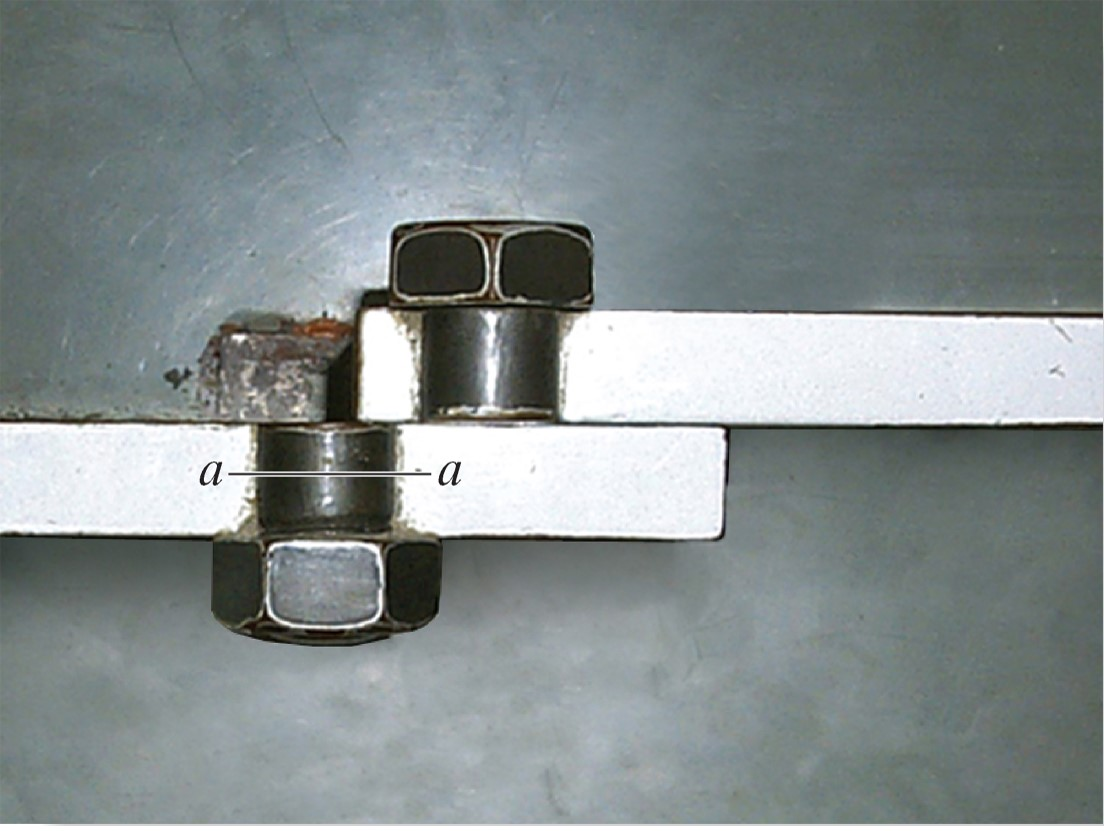
\includegraphics[width=0.6\linewidth]{bolt}
			\label{fig:bolt}
		\end{figure}

		\begin{figure}[H]
			\centering
			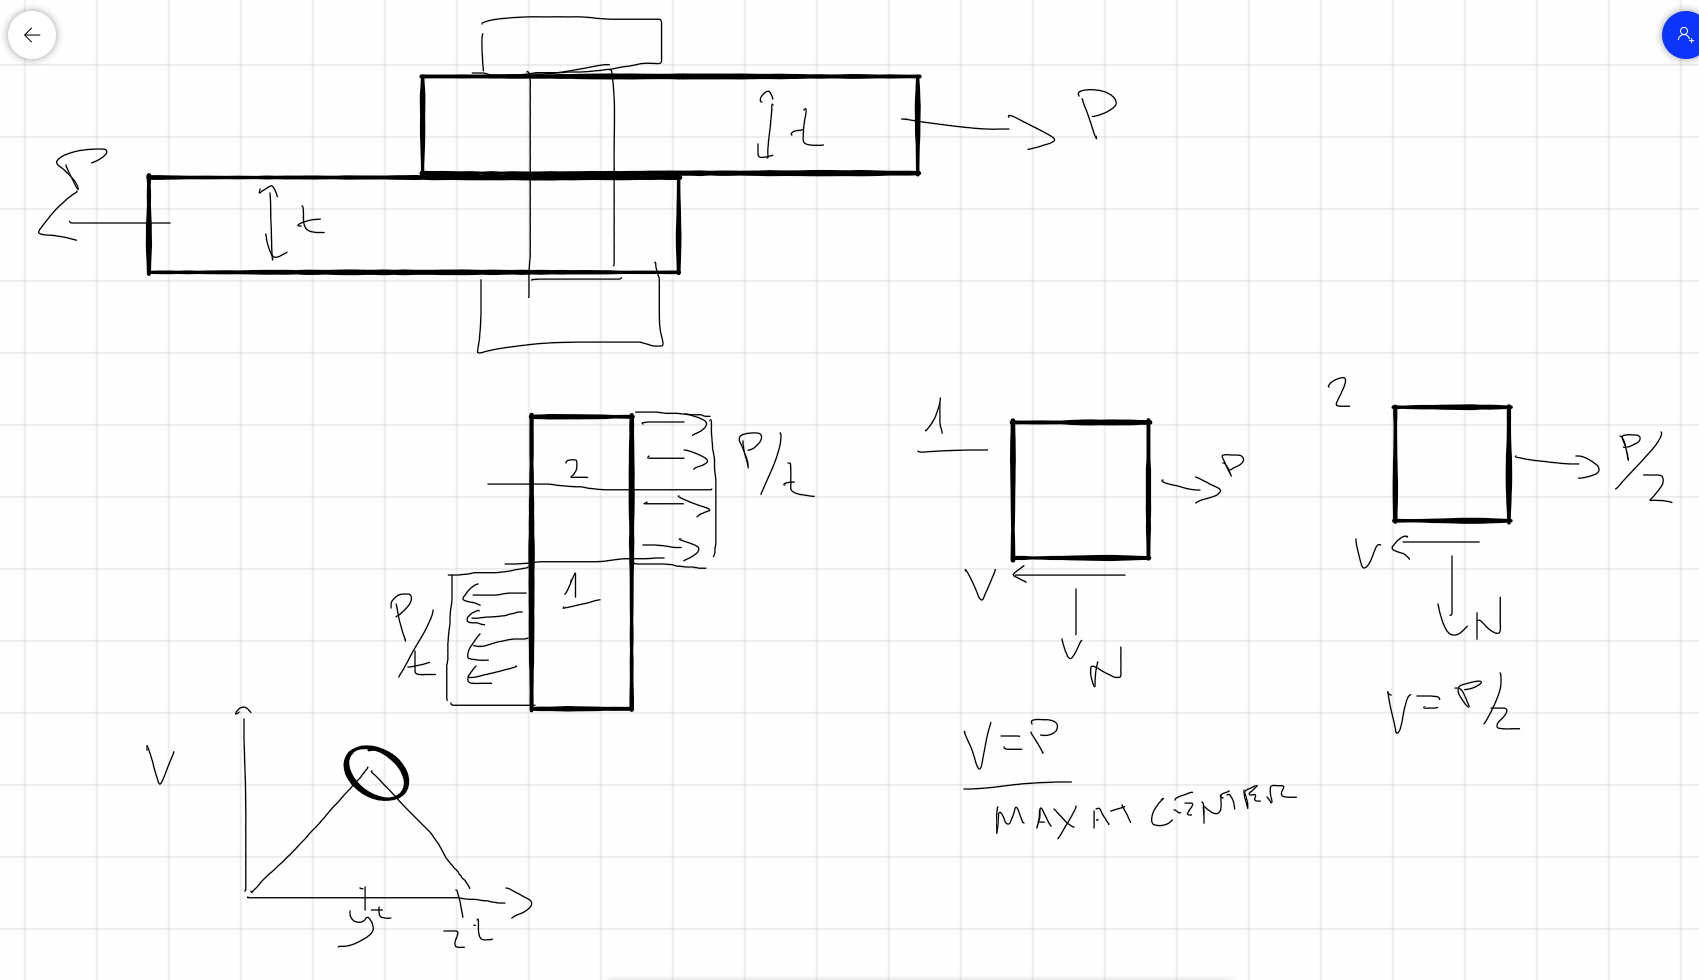
\includegraphics[width=0.8\linewidth]{hw1-9}
		\end{figure}

\end{enumerate}
\end{document}
